\section{Arrays}

\begin{frame}[fragile]
  \frametitle{Arrays: Introduction}
  \begin{itemize}
  \item Similar to lists, but homogeneous
  \item Much faster than arrays
  \end{itemize}
  \begin{lstlisting}
   In[]: a1 = array([1,2,3,4])
   In[]: a1 # 1-D
   In[]: a2 = array([[1,2,3,4],[5,6,7,8]])
   In[]: a2 # 2-D
  \end{lstlisting}
\end{frame}

\begin{frame}[fragile]
  \frametitle{\texttt{arange} and \texttt{shape}}
  \begin{lstlisting}
   In[]: ar1 = arange(1, 5)
   In[]: ar2 = arange(1, 9) 
   In[]: print ar2
   In[]: ar2.shape = 2, 4
   In[]: print ar2
  \end{lstlisting}
  \begin{itemize}
  \item \texttt{linspace} and \texttt{loadtxt} also returned arrays
  \end{itemize}
  \begin{lstlisting}
   In[]: ar1.shape
   In[]: ar2.shape
  \end{lstlisting}
\end{frame}

\begin{frame}[fragile]
  \frametitle{Special methods}
  \begin{lstlisting}
   In[]: identity(3)
  \end{lstlisting}
  \begin{itemize}
  \item array of shape (3, 3) with diagonals as 1s, rest 0s
  \end{itemize}
  \begin{lstlisting}
   In[]: zeros((4,5))
  \end{lstlisting}
  \begin{itemize}
  \item array of shape (4, 5) with all 0s
  \end{itemize}
  \begin{lstlisting}
   In[]: a = zeros_like([1.5, 1, 2, 3])
   In[]: print a, a.dtype
  \end{lstlisting}
  \begin{itemize}
  \item An array with all 0s, with similar shape and dtype as argument
  \item Homogeneity makes the dtype of a to be float
  \item \texttt{ones, ones\_like, empty, empty\_like}
  \end{itemize}
\end{frame}

\begin{frame}[fragile]
  \frametitle{Operations on arrays}
  \begin{lstlisting}
  In[]:  a1
  In[]:  a1 * 2
  In[]:  a1
  \end{lstlisting}
  \begin{itemize}
  \item The array is not changed; New array is returned
  \end{itemize}
  \begin{lstlisting}
   In[]: a1 + 3
   In[]: a1 - 7
   In[]: a1 / 2.0
  \end{lstlisting}
\end{frame}

\begin{frame}[fragile]
  \frametitle{Operations on arrays \ldots}
  \begin{itemize}
  \item Like lists, we can assign the new array, the old name
  \end{itemize}
  \begin{lstlisting}
   In[]: a1 = a1 + 2
   In[]: a1
  \end{lstlisting}
  \begin{itemize}
   \item \alert{Beware of Augmented assignment!}
  \end{itemize}
  \begin{lstlisting}
   In[]: a, b = arange(1, 5), arange(1, 5)
   In[]: print a, a.dtype, b, b.dtype
   In[]: a = a/2.0
   In[]: b /= 2.0
   In[]: print a, a.dtype, b, b.dtype
  \end{lstlisting}
  \begin{itemize}
  \item Operations on two arrays; element-wise
  \end{itemize}
  \begin{lstlisting}
   In[]: a1 + a1
   In[]: a1 * a2
  \end{lstlisting}
\end{frame}

\section{Accessing pieces of arrays}

\begin{frame}[fragile]
  \frametitle{Accessing \& changing elements}
  \begin{lstlisting}
  In[]:  A = array([12, 23, 34, 45, 56])

  In[]:  C = array([[11, 12, 13, 14, 15],
                    [21, 22, 23, 24, 25],
                    [31, 32, 33, 34, 35],
                    [41, 42, 43, 44, 45],
                    [51, 52, 53, 54, 55]])

   In[]: A[2]
   In[]: C[2, 3]
  \end{lstlisting}
  \begin{itemize}
  \item Indexing starts from 0
  \item Assign new values, to change elements
  \end{itemize}
  \begin{lstlisting}
   In[]: A[2] = -34
   In[]: C[2, 3] = -34
  \end{lstlisting}
\end{frame}

\begin{frame}[fragile]
  \frametitle{Accessing rows}
  \begin{itemize}
  \item Indexing works just like with lists
  \end{itemize}
  \begin{lstlisting}
   In[]: C[2]
   In[]: C[4]
   In[]: C[-1]
  \end{lstlisting}
  \begin{itemize}
  \item Change the last row into all zeros
  \end{itemize}
  \begin{lstlisting}
   In[]:  C[-1] = [0, 0, 0, 0, 0]
  \end{lstlisting}
  OR
  \begin{lstlisting}
   In[]: C[-1] = 0
  \end{lstlisting}
\end{frame}

\begin{frame}[fragile]
  \frametitle{Accessing columns}
  \begin{lstlisting}
  In[]:  C[:, 2]
  In[]:  C[:, 4]
  In[]:  C[:, -1]
  \end{lstlisting}
  \begin{itemize}
  \item The first parameter is replaced by a \texttt{:} to specify we
    require all elements of that dimension
  \end{itemize}
  \begin{lstlisting}
  In[]: C[:, -1] = 0
  \end{lstlisting}
\end{frame}

\begin{frame}[fragile]
  \frametitle{Slicing}
  \begin{lstlisting}
   In[]: I = imread('squares.png')
   In[]: imshow(I)
  \end{lstlisting}
  \begin{itemize}
  \item The image is just an array
  \end{itemize}
  \begin{lstlisting}
   In[]: print I, I.shape
  \end{lstlisting}
  \begin{enumerate}
  \item Get the top left quadrant of the image
  \item Obtain the square in the center of the image
  \end{enumerate}
\end{frame}

\begin{frame}[fragile]
  \frametitle{Slicing \ldots}
  \begin{itemize}
  \item Slicing works just like with lists
  \end{itemize}
  \begin{lstlisting}
  In[]: C[0:3, 2]
  In[]: C[2, 0:3]
  In[]: C[2, :3]
  \end{lstlisting}
  \begin{lstlisting}
  In[]: imshow(I[:150, :150])

  In[]: imshow(I[75:225, 75:225])
  \end{lstlisting}
\end{frame}

\begin{frame}
\frametitle{Image after slicing}
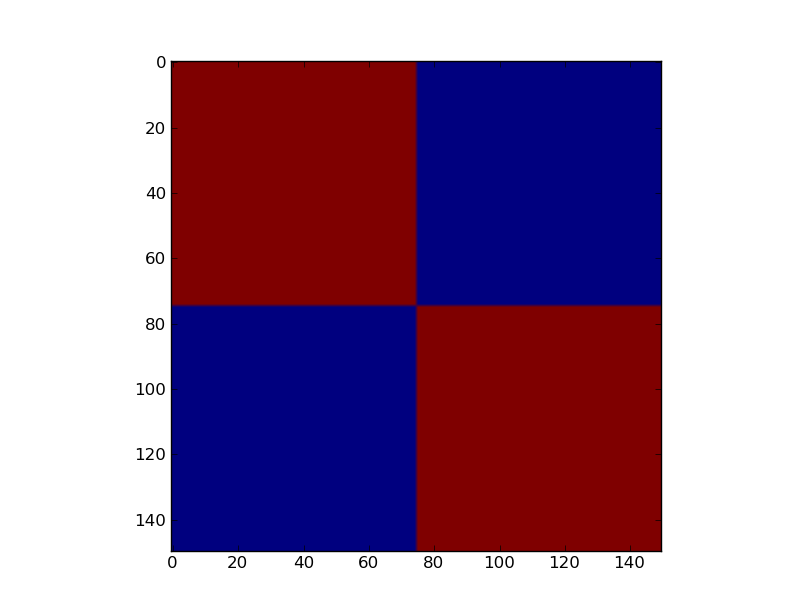
\includegraphics[scale=0.45]{../advanced_python/images/slice.png}\\
\end{frame}



\begin{frame}[fragile]
  \frametitle{Striding}
  \begin{itemize}
  \item Compress the image to a fourth, by dropping alternate rows and
    columns
  \item We shall use striding
  \item The idea is similar to striding in lists
  \end{itemize}
  \begin{lstlisting}
  In[]: C[0:5:2, 0:5:2]
  In[]: C[::2, ::2]
  In[]: C[1::2, ::2]
  \end{lstlisting}
  \begin{itemize}
  \item Now, the image can be shrunk by
  \end{itemize}
  \begin{lstlisting}
  In[]: imshow(I[::2, ::2])
  \end{lstlisting}
\end{frame}

\section{Matrix Operations}

\begin{frame}[fragile]
  \frametitle{Matrix Operations using \texttt{arrays}}
  We can perform various matrix operations on \texttt{arrays}\\ 
  A few are listed below.

  \begin{center}
    \begin{tabular}{lll}
      Operation                    &  How?           &  Example           \\
      \hline
      Transpose                    &  \texttt{.T}       &  \texttt{A.T}         \\
      Product                      &  \texttt{dot}      &  \texttt{dot(A, B)}   \\
      Inverse                      &  \texttt{inv}      &  \texttt{inv(A)}      \\
      Determinant                  &  \texttt{det}      &  \texttt{det(A)}      \\
      Sum of all elements          &  \texttt{sum}      &  \texttt{sum(A)}      \\
      Eigenvalues                  &  \texttt{eigvals}  &  \texttt{eigvals(A)}  \\
      Eigenvalues \& Eigenvectors  &  \texttt{eig}      &  \texttt{eig(A)}      \\
      Norms                        &  \texttt{norm}     &  \texttt{norm(A)}     \\
      SVD                          &  \texttt{svd}      &  \texttt{svd(A)}      \\
    \end{tabular}
  \end{center}
\end{frame}

\section{Least square fit}

\begin{frame}[fragile]
  \frametitle{Least Square Fit}
  \begin{lstlisting}
  In[]:  L, t = loadtxt("pendulum.txt", 
                unpack=True)
  In[]:  L
  In[]:  t
  In[]:  tsq = t * t
  In[]:  plot(L, tsq, 'bo')
  In[]:  plot(L, tsq, 'r')
  \end{lstlisting}
  \begin{itemize}
  \item Both the plots, aren't what we expect -- linear plot
  \item Enter Least square fit!
  \end{itemize}
\end{frame}

\begin{frame}[fragile]
  \frametitle{Matrix Formulation}
  \begin{itemize}
  \item We need to fit a line through points for the equation $T^2 = m \cdot L+c$
  \item In matrix form, the equation can be represented as $T_{sq} = A \cdot p$, where $T_{sq}$ is
    $\begin{bmatrix}
    T^2_1 \\
    T^2_2 \\
    \vdots\\
    T^2_N \\
  \end{bmatrix}$
    , A is   
    $\begin{bmatrix}
    L_1 & 1 \\
    L_2 & 1 \\
    \vdots & \vdots\\
    L_N & 1 \\
  \end{bmatrix}$
    and p is 
    $\begin{bmatrix}
      m\\
      c\\
    \end{bmatrix}$
  \item We need to find $p$ to plot the line
  \end{itemize}
\end{frame}

\begin{frame}[fragile]
  \frametitle{Least Square Fit Line}
  \begin{lstlisting}
  In[]:  A = array((L, ones_like(L)))
  In[]:  A.T
  In[]:  A
  \end{lstlisting}
  \begin{itemize}
  \item We now have \texttt{A} and \texttt{tsq}
  \end{itemize}
  \begin{lstlisting}
  In[]: result = lstsq(A, tsq)
  \end{lstlisting}
  \begin{itemize}
  \item Result has a lot of values along with m and c, that we need
  \end{itemize}
  \begin{lstlisting}
  In[]: m, c = result[0]
  In[]: print m, c
  \end{lstlisting}
\end{frame}

\begin{frame}[fragile]
  \frametitle{Least Square Fit Line}
  \begin{itemize}
  \item Now that we have m and c, we use them to generate line and plot
  \end{itemize}
  \begin{lstlisting}
  In[]:  tsq_fit = m * L + c
  In[]:  plot(L, tsq, 'bo')
  In[]:  plot(L, tsq_fit, 'r')
  \end{lstlisting}
\end{frame}

\begin{frame}
\frametitle{Least Square Fit Line}
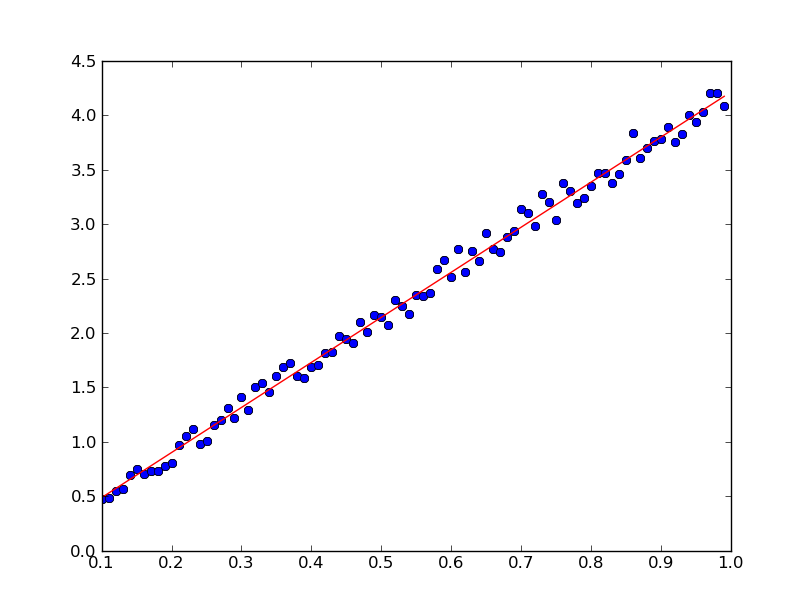
\includegraphics[scale=0.45]{../advanced_python/images/lst-sq-fit.png}\\
\end{frame}


